\section{Hidden comunication by targeted reflections}

We will start from the paper \textit{Reconfigurable Intelligent Surface: Reflection Design Against Passive Eavesdropping} \cite{9328149}, explaining how to hide communication between two actors from eavesdroppers using Reconfigurable Intelligent Surfaces, then expanding it to multiple receiving users at the same time.

\subsection{The paper problem mathematics}

\begin{figure}[H]
  \centering
  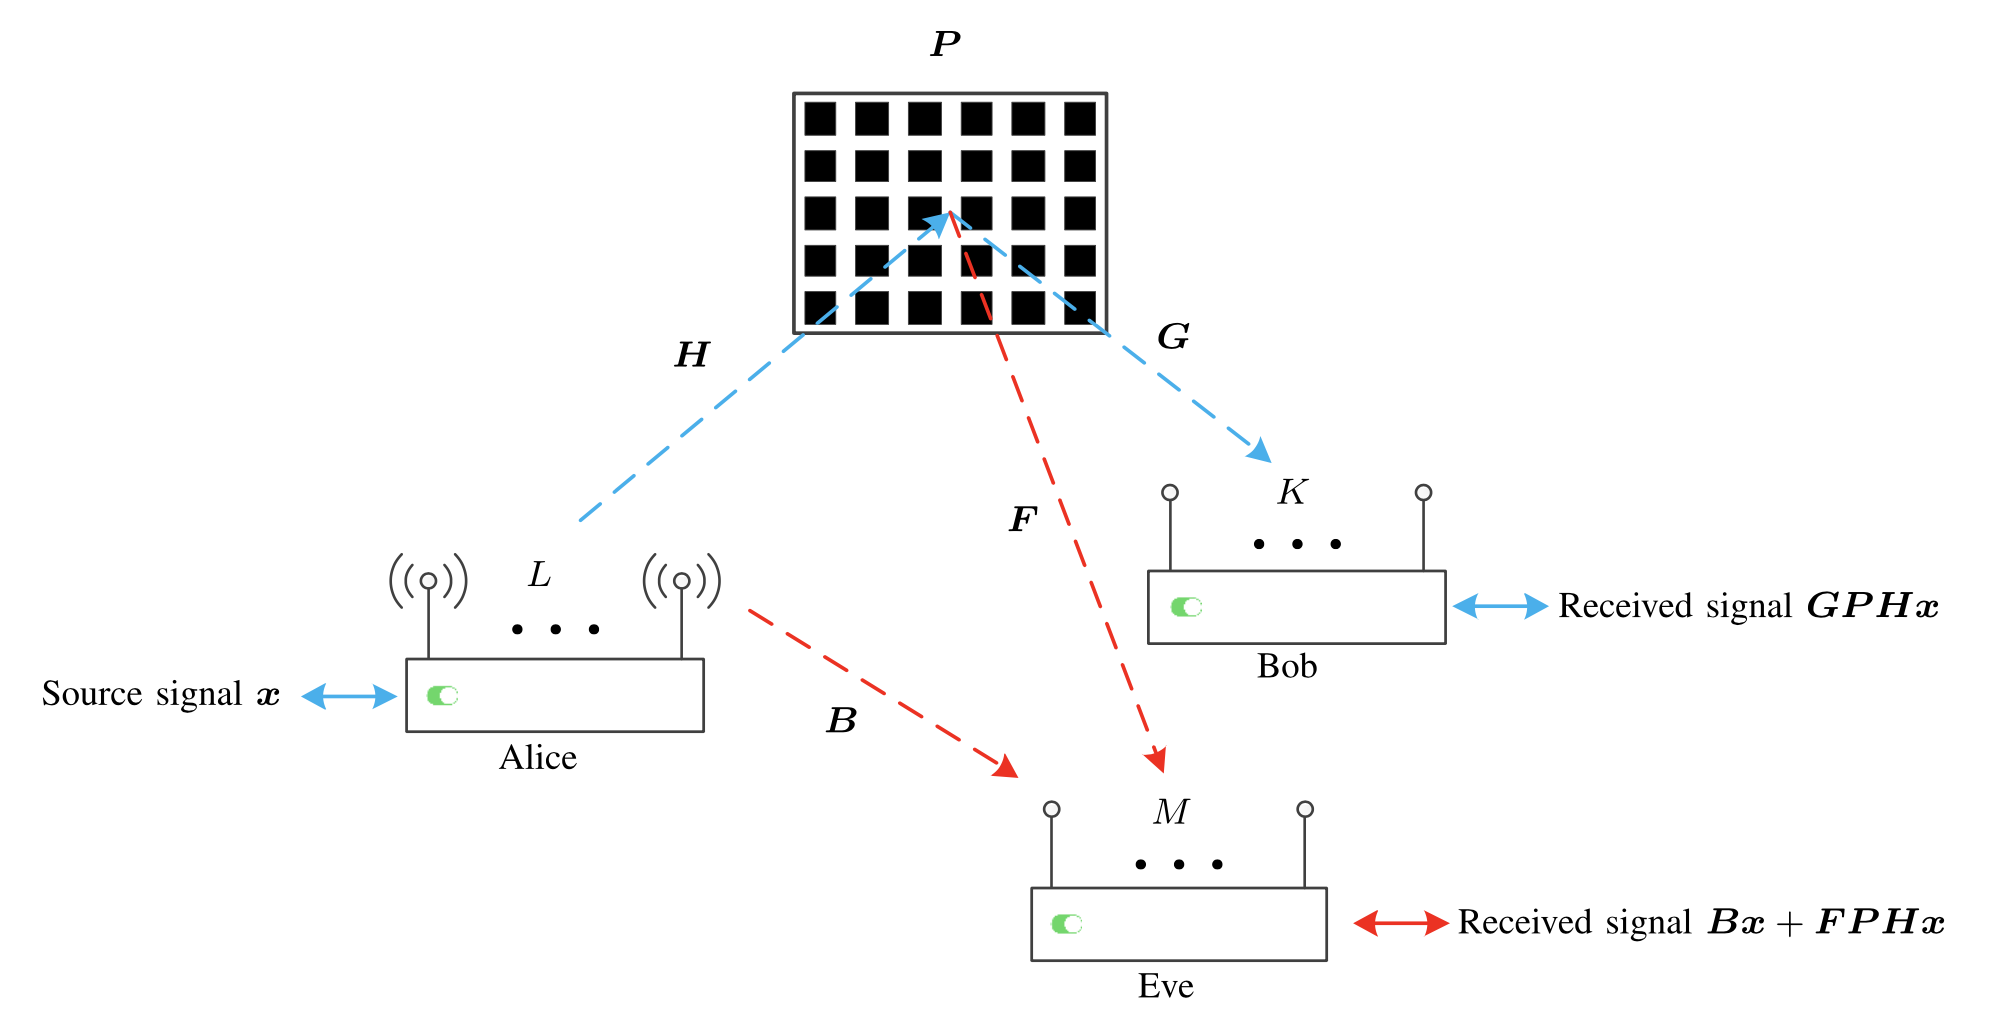
\includegraphics[width=\linewidth]{imgs/problem-description.png}
  \caption{Setup}
  \label{fig:correlation_sk}
\end{figure}

In \cite{9328149}, the authors studied how to use RISs to allow communications between two users without LOS, while making the signal undeciphrable for eavesdroppers. We call $L$ the transmitter's antennas, $K$ the receiver's antennas, $M$ the eavesdropper's antenna, and $N$ the RIS reflecting elements. We assume $L \ge K \ge 2$.

We define $H \in \C^{NxL}$ the channel response from the transmitter to the RIS, $G \in \C^{KxN}$ the channel response from the RIS to the receiver, $P = diag\{p\} \in \C^{NxN}$ a diagonal matrix in which the $n$th diagonal element represents the reflection coefficient of the $n$th unit at the RIS.

The objective is making the receiver's final signal $GPH$ a diagonal matrix, while making every possible eavesdropper's final signal a full matrix.

We will leave for now the technical details of why this would achieve secrecy for the legitimate users to the original paper, and will just focus on the mathematics behind the calculation. Our final objective will be to generalize these calculations to $J$ receving users and multiple RISs used in parallel and in sequence.

Formally, the condition we want to satisfy is:

\begin{equation}
  || [GPH]_{:,1:K} - [[GPH]_{:,1:K}]_{diag} || ^2 = 0
\end{equation}

Where $[GPH]_{:,1:K} \in \C^{KxK}$ denotes the first K columns of the matrix $GPH \in \C^{KxL}$.

Given

\begin{equation}
  W = \sum_{i,j = 1, i \ne j}^{K} (g_{j,:} \odot h_i^T)^H (g_{j,:} \odot h_i^T)
\end{equation}

The formula (1) can be rewritten as

\begin{equation}
  Wp = 0
\end{equation}

and the solutions of $p$ can be found in the null space of $W$. Using singular value decomposition (SVD), we can decompose

\begin{equation}
  W = R \lambda V^H
\end{equation}

Taken $U \in \C ^ {Nx(N-(K^2 - K))}$ the last $N-(K^2 - K)$ columns of the left singular matrix $R$. We then have

\begin{equation} p = Uq \end{equation}

and

\begin{equation}WU = 0\end{equation}

[TODO: EXPLANATION AND CITATION NEEDED], so all together we have

\begin{equation}
  WUq = 0
\end{equation}

being true, and $q \in \C^{N-(K^2 - K)}$ can be a random vector.